\chapter{Relation Between Several Variables}

When we have two groups, we can ask the question: "Are they different?" The answer is provided by hypothesis tests: by a \emph{t-test} if the data are normally distributed, or by a \emph{Mann-Whitney test} otherwise. If we want to go one step further and predict the value of one variable from another, we have to use the technique of \emph{linear regression}.

So what happens when we have more than two groups?

To answer the question "Are they different?" for more than two groups, we have to use the \emph{Analysis of Variance (ANOVA)-test} for data where the residuals are normally distributed. If this condition is not fulfilled, the \emph{Kruskal-Wallis Test} has to be used.

What should we do if we have paired data?

If we have matched pairs for two groups, and the differences are not normally distributed, we can use the \emph{Wilcoxon signed rank sum test}. The rank test for more than two groups of matched data is the \emph{Friedman test}\index{general}{test!Friedman}.\footnote{It may be worth mentioning that Thom Baguley suggested the following: Where one-way repeated measures ANOVA is not appropriate, rank transformation followed by ANOVA will provide a more robust test with greater statistical power than the Friedman test.}

An example for the application of the Friedman test: Ten professional piano players are blindfolded, and are asked to judge the quality of three different pianos. Each player rates each piano on a scale of 1 to 10 (1 being the lowest possible grade, and 10 the highest possible grade). The null hypothesis is that all three pianos rate equally. To test the null hypothesis, the Friedman test is used on the ratings of the ten piano players.

When moving from two to many variables, the correlation coefficient gets replaced by the \emph{correlation matrix}\index{general}{correlation matrix}. And if we want to and predict the value of \emph{many} other variables, linear regression has to be replaced by \emph{multilinear regression}\index{general}{regression!multilinear}, sometimes also referred to as \emph{multiple linear regression}.

However, watch out for the pitfalls that loom when you work with many variables! Take for example the following hypothetical case: you make a survey about the activity and life circumstances of a large range of people, covering all the numbers that you can get your hand on. In this survey you find out that a) rich people spend more time playing golf than poor people, and b) rich people tend to have fewer children than poor people. This leads to a strong negative correlation between playing golf and having children, and you may be tempted to (falsely) draw the conclusion that playing golf reduces your fertility, while in reality it is the higher income which causes both effects. \cite{Kaplan2009} nicely describes where those problems come from, and how best to avoid them.

\section{Two-way ANOVA} \label{sec:anovaTwoWay} \index{general}{ANOVA!two-way} \index{general}{test!ANOVA}

Compared to one-way ANOVAs, the analysis with two-way ANOVAs has a new element. We can look not only if each of the factors is significant; we can also check if the \emph{interaction} of the factors has a significant influence on the distribution of the data. For sticking to the example above, if only women with treatment B get healthy, we have a significant interaction effect between "gender" and "treatment".

\PyImg "anovaTwoway.py" (p \pageref{py:anovaTwoway}): Two-way Analysis of Variance (ANOVA).
\index{python}{anovaTwoway}

\begin{verbatim}
                        df  sum_sq mean_sq        F    PR(>F)
  C(fetus)               2  324.00  162.00  2113.10  1.05e-27
  C(observer)            3    1.19    0.39     5.21  6.497-03
  C(fetus):C(observer)   6    0.56    0.09     1.22  3.29e-01
  Residual              24    1.84    0.07      NaN       NaN
\end{verbatim}

\section{Three-way ANOVA} \label{sec:anovaThreeWay} \index{general}{ANOVA!three-way}

When you have more than two factors, it is recommendable to use \emph{statistical modeling} for the data analysis (see Chapter \ref{chapter:Models}). However, as always with the analysis of statistical data, you should first inspect the data visually. \emph{seaborn} makes this quite simple:

\begin{figure}
  \centering
  \includegraphics[width=0.75\textwidth]{../Images/ANOVA_3way.png}\\
  \caption{Three-way ANOVA.}\label{fig:ANOVA3way}
\end{figure}

\begin{lstlisting}
    import matplotlib.pyplot as plt
    import seaborn as sns
    sns.set(style="whitegrid")

    df = sns.load_dataset("exercise")

    sns.factorplot("time", "pulse", hue="kind", col="diet", data=df,
                   hue_order=["rest", "walking", "running"],
                   palette="YlGnBu_d", aspect=.75).despine(left=True)
    plt.show()
\end{lstlisting}

\section{Visualization of Multivariate Correlations}

\subsection{Scatterplot Matrix}\index{general}{Scatterplot matrix}

If you have three to six variables that may be related to each other, you can use a "scatterplot matrix" to visualize the different correlations:

\begin{lstlisting}
    import seaborn as sns
    sns.set()

    df = sns.load_dataset("iris")
    sns.pairplot(df, hue="species", size=2.5)
\end{lstlisting}

\begin{figure}
  \centering
  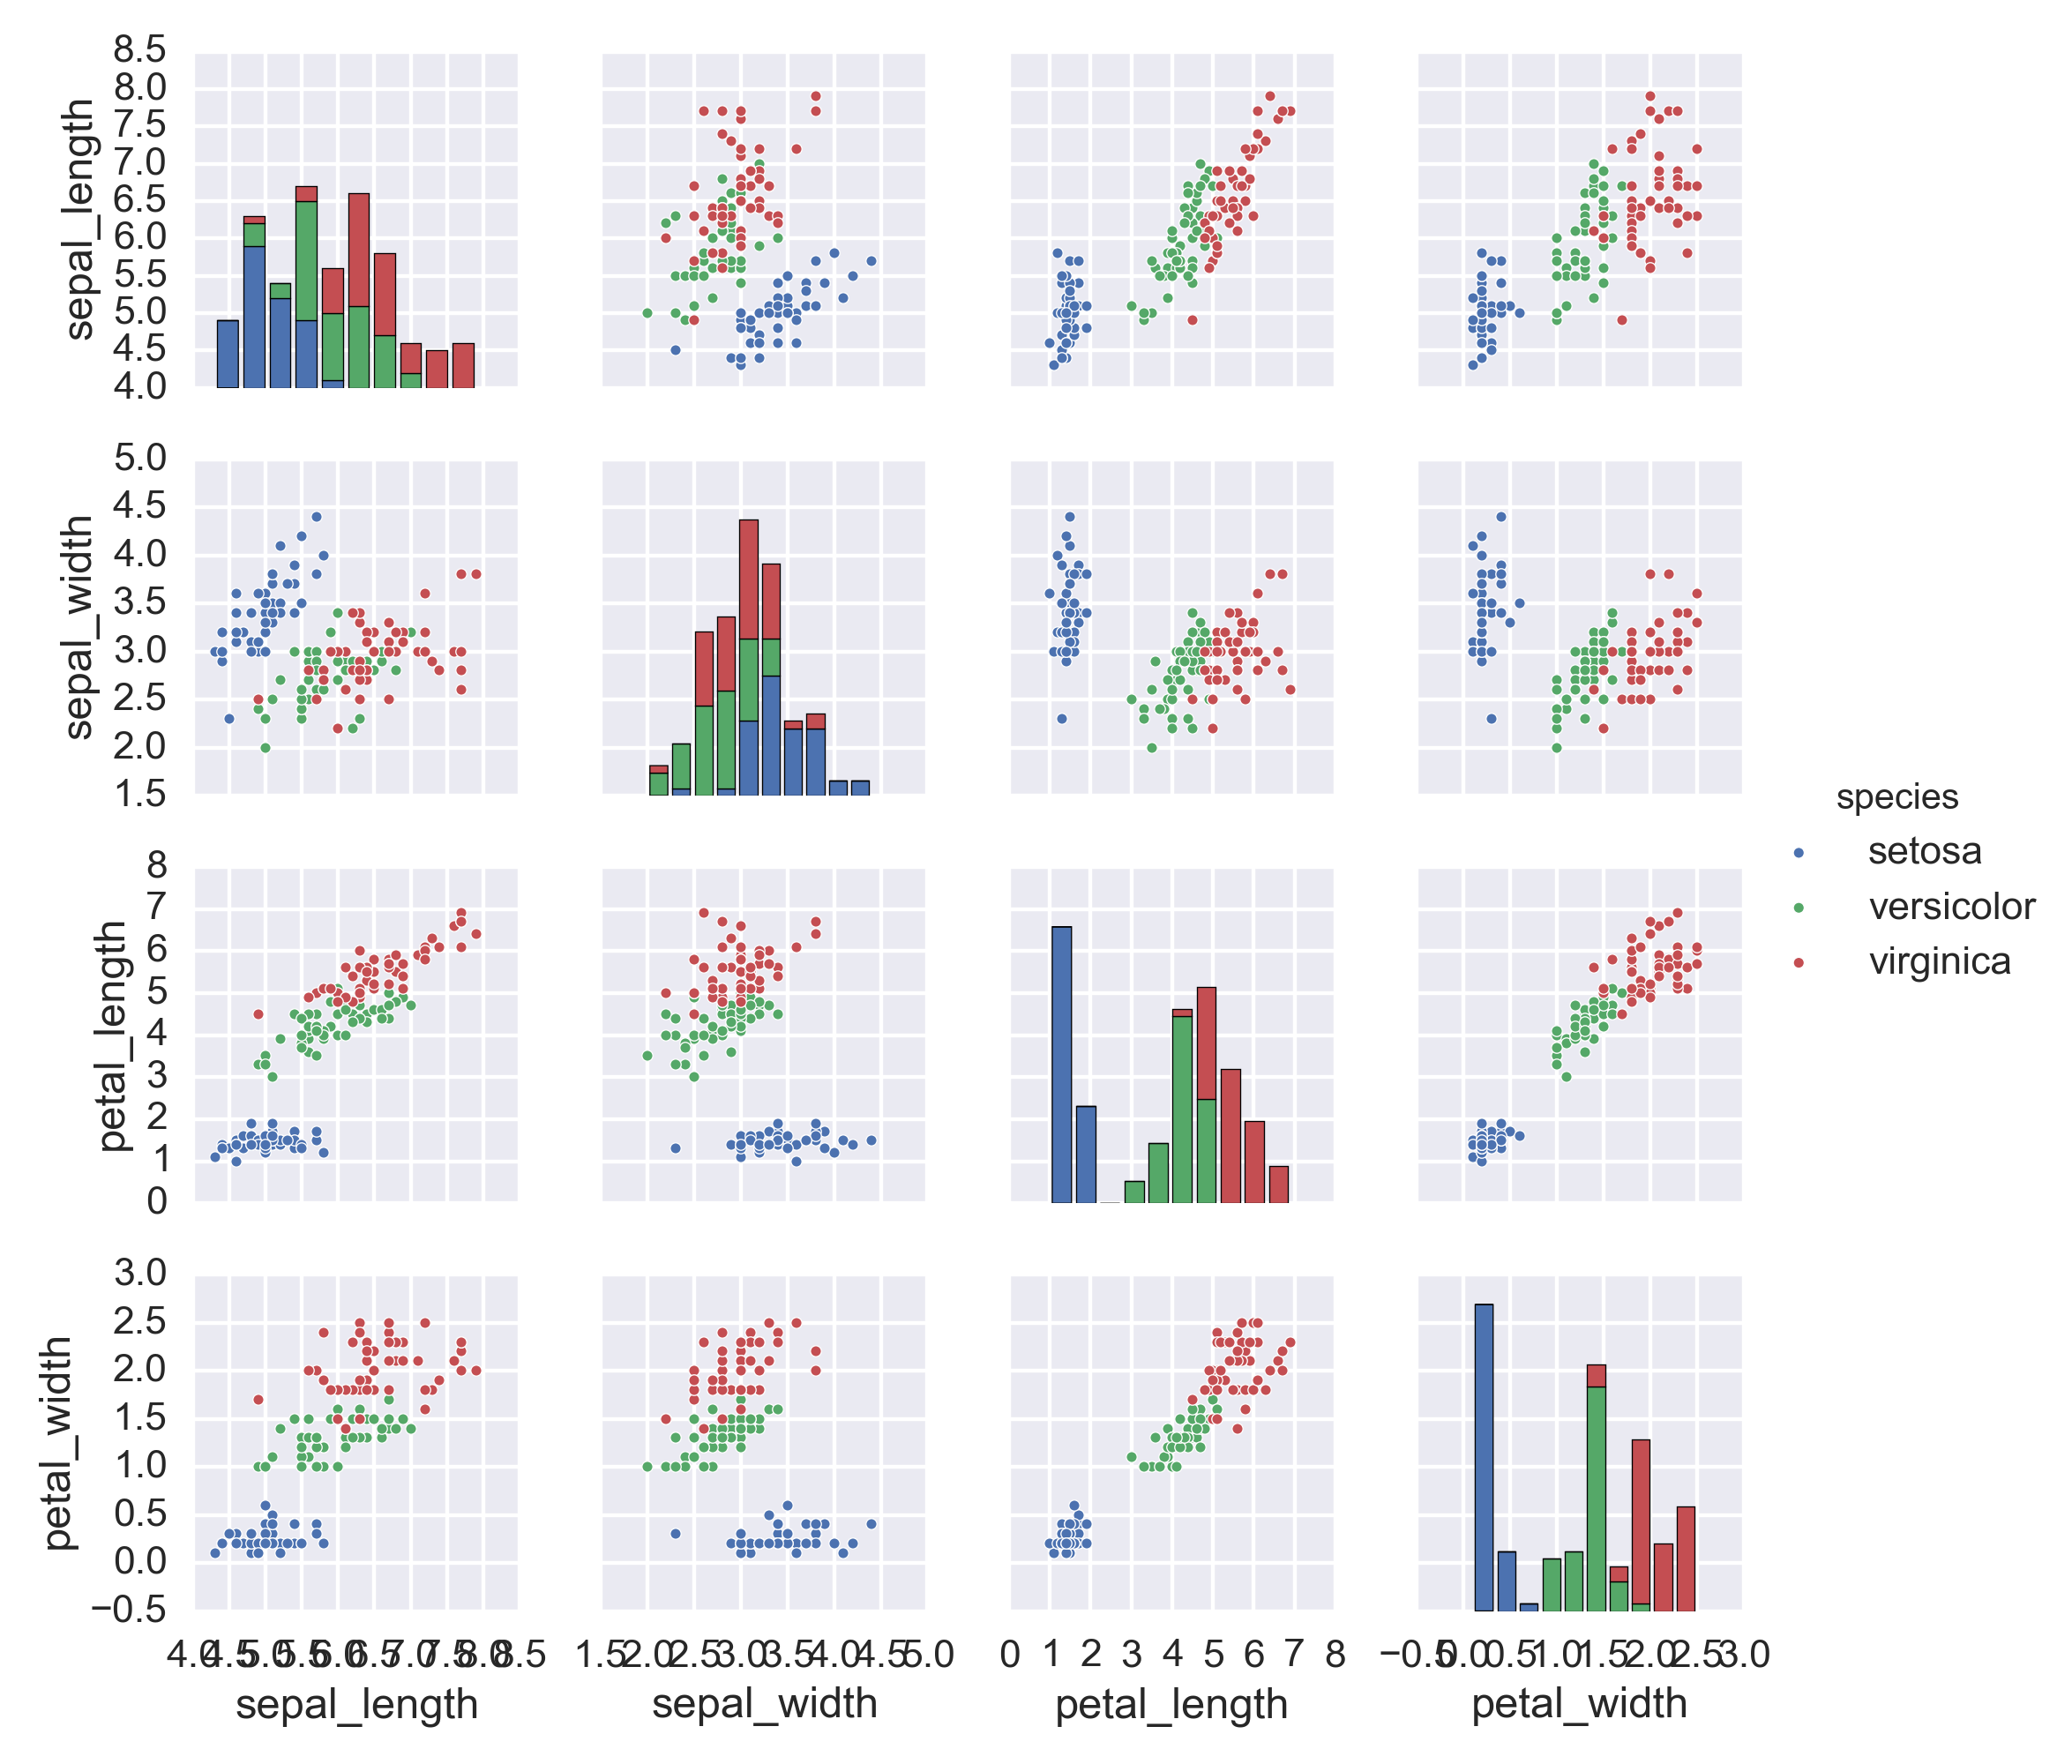
\includegraphics[width=0.85\textwidth]{../Images/multiScatterplot.png}\\
  \caption{Scatterplot matrix.}\label{fig:scatterplotMatrix}
\end{figure}


\subsection{Correlation Matrix}\index{general}{Correlation matrix}

An elegant way to visualize the correlation between a large number of variables is the \emph{correlation matrix}. Using \emph{seaborn}, it can be implemented elegantly as follows:

\begin{figure}
  \centering
  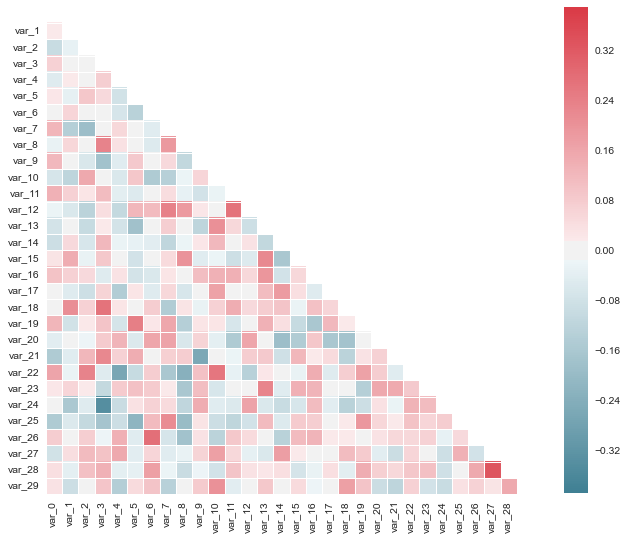
\includegraphics[width=0.75\textwidth]{../Images/many_pairwise_correlations.png}\\
  \caption{Visualization of the Correlation matrix.}\label{fig:CorrelationMatrix}
\end{figure}

\begin{lstlisting}
    import numpy as np
    import seaborn as sns
    import matplotlib.pyplot as plt
    sns.set(style="darkgrid")

    rs = np.random.RandomState(33)
    d = rs.normal(size=(100, 30))

    f, ax = plt.subplots(figsize=(9, 9))
    cmap = sns.diverging_palette(220, 10, as_cmap=True)
    sns.corrplot(d, annot=False, sig_stars=False,
                 diag_names=False, cmap=cmap, ax=ax)
    f.tight_layout()
\end{lstlisting}


\section{Multilinear Regression} \index{general}{regression!multilinear}

If you have truly independent variables, \emph{multilinear regression} is a straightforward extension of the simple linear regression.

\paragraph{Multiple Regression} \index{general}{regression!multiple}
Example of \emph{multiple regression} with covariates (i.e. independent variables) $w_i$ and $x_i$.
Again suppose that the data are 7 observations, and for each observed value to be predicted ($y_i$) there are two covariates that were also observed, $w_i$ and $x_i$. The model to be considered is

\begin{equation}
  y_i = \beta_0 + \beta_1 w_i + \beta_2 x_i + \epsilon_i
\end{equation}

This model can be written in matrix terms as

\begin{equation}\label{eq:multipleRegression}
  \begin{bmatrix}y_1 \\ y_2 \\ y_3 \\ y_4 \\ y_5 \\ y_6 \\ y_7 \end{bmatrix} =
    \begin{bmatrix} 1 & w_1 & x_1  \\1 & w_2 & x_2  \\1 & w_3 & x_3  \\1 & w_4 & x_4  \\1 & w_5 & x_5  \\1 & w_6 & x_6 \\ 1& w_7  & x_7  \end{bmatrix}
    \begin{bmatrix} \beta_0 \\ \beta_1 \\ \beta_2  \end{bmatrix}
    +
    \begin{bmatrix} \epsilon_1 \\ \epsilon_2 \\ \epsilon_3 \\ \epsilon_4 \\ \epsilon_5 \\ \epsilon_6 \\ \epsilon_7 \end{bmatrix}
\end{equation}


However, you have to watch out: if your variables may be related to each other, you have to proceed much more carefully. For example, you may want to investigate how the prevalence of some disease correlates with age and with income: if you do so, you have to keep in mind that age and income are most likely correlated! For details, \cite{Kaplan2009} gives a good introduction to that topic. Also, check out the chapter on Modeling.

\PyImg "multipleRegression.py" (p \pageref{py:multipleRegression}): Multiple regression example.
\index{python}{multipleRegression} 